\section{Implementation} \label{sec:implementation}
\subsection{Registers} \label{sec:implementation:registers}
This chapter will explain the implementation details of the register-module: the architecture of the driver module, data-pointer register, data, stack, loop-skip, instruction, instruction-pointer, and flag register. At the end of this chapter, we will provide the entire picture of the register-module.

\subsubsection{Overview}
In BFCPU, we omitted ALU because the only mathematical operation that brainf*ck can perform is adding and subtracting one. For the sake of simplicity, we decided to utilize 74LS193 and 74LS161 integrated chips to make individual registers. Both chips provide memory functionality along with incrementing of the value. Additionally, 74LS193 provides decrementing of the current value stored in the chip. It is important to note that F-R does not need any increment-decrement (INC-DEC) functionality. Thus, we used 74LS*** since it provides only the storage of a 4-bit value. 

\subsubsection{Common INC-DEC functionality problem}
Register module possesses a lot of INC and DEC pins that the control unit needs to manipulate in order to alter the value of registers. Driver module removes this inconvenience and serves as the common interface for all registers, and thus the entire register-module. The idea behind driver module is limiting all INC and DEC pins to one DEC pin and one CE (count enable) pin, along with CLK (clock). If CE is HIGH, then based on the value of DEC pin, we can either decrement or increment on the rising edge of the clock pulse (CLK). The output of the driver module is the pair UP-DOWN that must be transmitted to an appropriate register\footnote{Or just UP signal for registers with 74LS161, as this chip can only increment}. Hence, we need a selecting interface to choose what register the computer is dealing with. The inner circuitry (see figure \ref{driver-module-arch}) accomplished this goal. A very general overview of the register-module is shown in the figure below. There are three select pins that provide us with 8 different possible paths, which is sufficient because we have less than 8 different registers.

\begin{figure}[H]
	\centering
	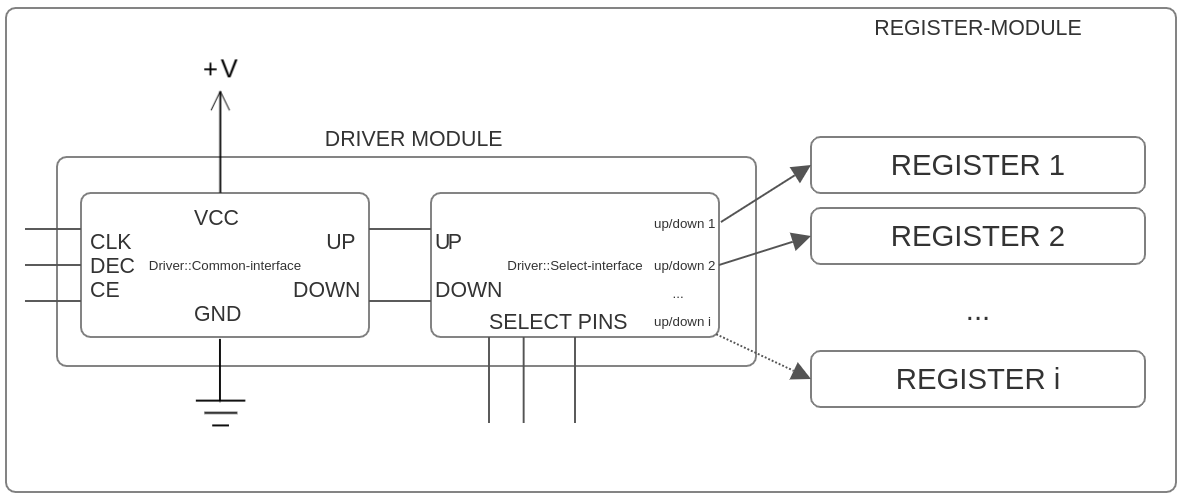
\includegraphics[width=0.9\textwidth]{img/register_module_overview}
	\caption{Register-module Overview}
	\label{fig:registerModuleOverview}
\end{figure}

\subsubsection{74LS193 Chaining}
Registers use 74LS193 (or 74LS161) to obtain storage and INC-DEC functionality. However, one 74LS193 chip has 4 bits whereas registers require 8 and 16 bits. Fortunately, 74LS193\footnote{Similar configuration works out for 74LS161, so we will not discuss it here} has a chaining ability: if CO (carry out) is connected to the UP pin of the other chip, and BO (borrow out) is connected to the DOWN pin, then we will obtain more bits available (see figure \ref{fig:registerModuleChaining}). This technique is used in every register that requires more than 4 bits.

\begin{figure}[H]
	\centering
	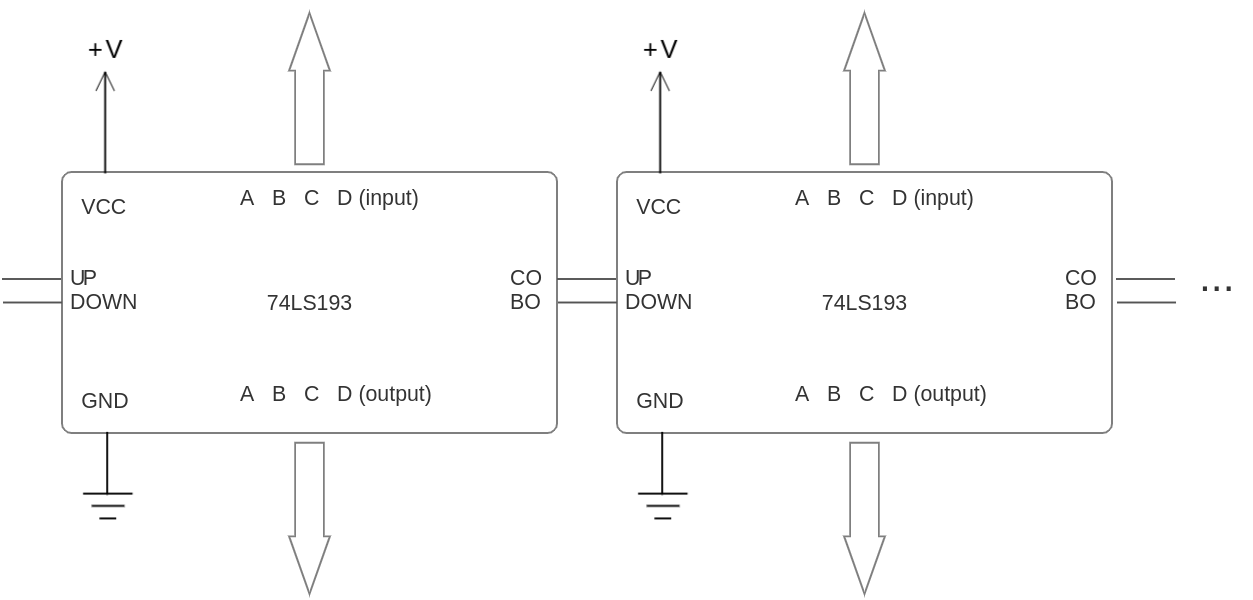
\includegraphics[width=0.9\textwidth]{img/register_module_chaining}
	\caption{Register-module 74LS193 chaining}
	\label{fig:registerModuleChaining}
\end{figure}

\subsubsection{Circuit: Driver Module}
As visible from figure \ref{fig:registerModuleOverview}, the driver module has two parts: common interface, select interface. Connection to registers is the bridge between the driver module and registers in the register module.

We used two demuxers to create the common interface. The basic idea behind this implementation is the following: DEC pin defines the way where CE and CLK signals are propagated, so DEC is connected to the select pin of both demuxers. CE switches the signals off or on, while CLK stimulates the alterations in UP/DOWN pairs, contributing to the change in the value of a register. 

Because of the inner circuit of 74LS193, we need to avoid simultaneous pulsing and UP/DOWN pair grounded since it unfavorably alters the value of a register. The solution was quite straightforward: CLK pin of the driver module is connected to the output of anded clock signal and CE pin. 

The resulting UP/DOWN pair is directed to the select interface, that redirects the pair to a specific, selected, register. This behavior is accomplished by utilizing 3-to-8 demuxers, because we have less than 8 registers but more than 4.

\begin{figure}[H]
	\centering
	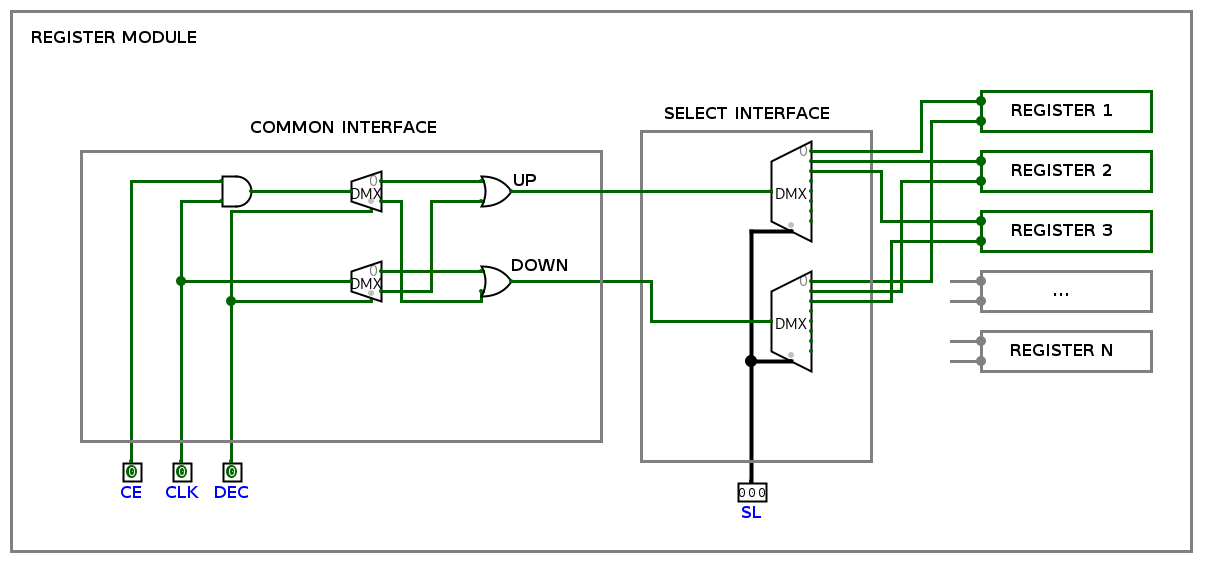
\includegraphics[width=0.9\textwidth]{img/driver_module_implementation}
	\caption{Driver Module Implementation}
	\label{fig:driverModuleImplementation}
\end{figure}



\subsubsection{Circuit: Data Register}
Data register is a 8-bit valued flip-flop with both increment and decrement functionality. Therefore, we used 74LS193 chip. One essential property of the data register is that it also outputs a so-called zero flag (Z), which is 1 only if stored value is 0. The latter ability is implemented using OR gates and direct connection to stored bits. (see figure \ref{fig:dataRegisterImplementation})

\begin{figure}[H]
	\centering
	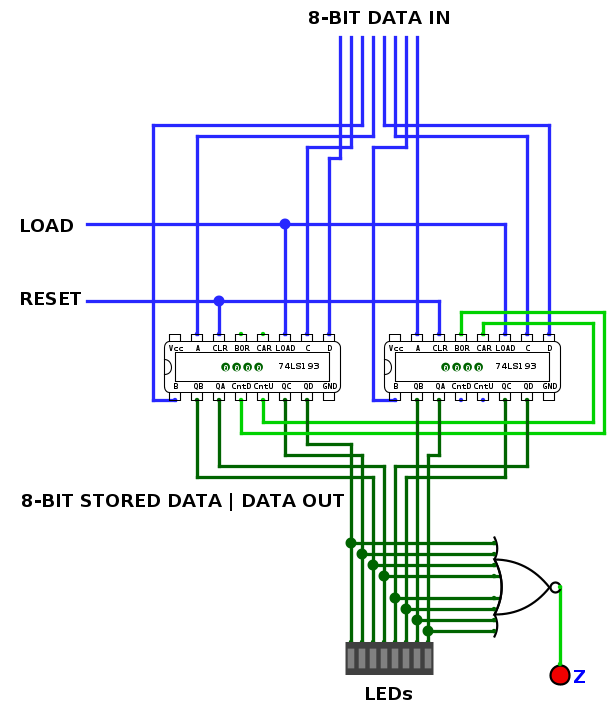
\includegraphics[width=0.9\textwidth]{img/data_register_implementation}
	\caption{Data Register Implementation}
	\label{fig:dataRegisterImplementation}
\end{figure}


\subsubsection{Circuit: Data-Pointer Register}
Data-Pointer register is a 8-bit valued flip-flop with both increment and decrement functionality. Therefore, we used 74LS193 chip. There is nothing very special about the data-pointer register, except that its output (value stored inside) is connected to the bus transceiver, but this applies for other registers as well\footnote{Implementation of the bus transceiver is fairly straightforward: as only outputs are connected along with DIR and CE (chip enable) pins as an input. Chips used is 74LS245}. (see figure \ref{fig:dataPointerRegisterImplementation})

\begin{figure}[H]
	\centering
	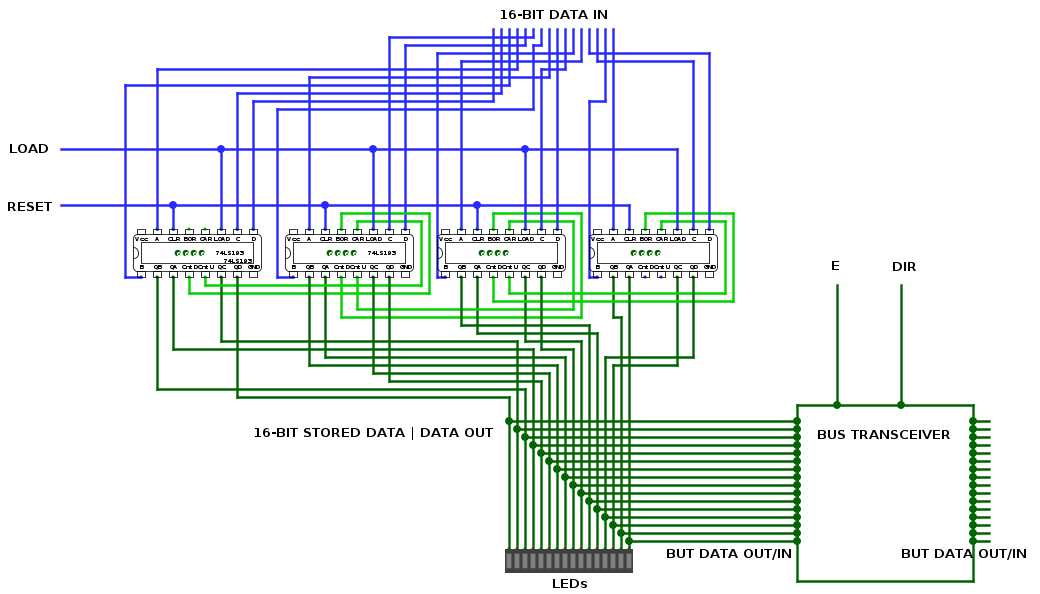
\includegraphics[width=0.9\textwidth]{img/data_pointer_register_implementation}
	\caption{Data-Pointer Register Implementation}
	\label{fig:dataPointerRegisterImplementation}
\end{figure}

\subsubsection{Circuit: Loop-Skip Register}

\subsubsection{Circuit: Instruction Register}

\subsubsection{Circuit: Instruction-Pointer Register}

\subsubsection{Circuit: Stack Register}

\subsubsection{Circuit: Flag Register}



\subsection{Memory}
\subsection{Control Unit}
\subsection{Input}
\subsection{Output}

